\subsection{The models}

	For all the datasets a model with the following configuration has been trained. The inputs of the model are the PL intensities and the outputs are the flattened matrices that represent the PSFs' complex fields.\\
	
	{\normalsize HYPERPARAMETERS:}
	\begin{lstlisting}
	*ARCHITECTURE HYPERPARAMETERS:
		-Fully Connected
		-Input shape: 19
		-Output shape: 
			- 32768 for original sized PSF electric field
			- 16384 for original sized PSF intensity 
			- 8192 for cropped sized PSF electric field
			- 4096 for cropped sized PSF intensity 
		-Hidden layers: [1024, 1024, 1024, 1024, 1024, 1024]
		-Regularizer: None
		-Hidden Layers Activation: relu
		-Output Layer Activation: linear
		-Batch Normalization: False
		-Dropout: False, 0.2
	
	*COMPILATION HYPERPARAMETERS:
		-Optimizer: ADAM lr=0.001, beta_1=0.9, beta_2=0.999
		-Loss Function: MSE
		-Metric: MSE
	
	*TRAINING HYPERPARAMETERS:
		-Epochs: 100
		-Batch size: 32
		-Callbacks: 
			-ReduceLROnPlateau: MSE 20 x0.1
			-Early Stop: MSE 50
	\end{lstlisting}
	
	The exception is the model trained for the Atmospheric Aberration Cropped PSF which has Batch Normalization activated.
	
	\subsubsection{Atmospheric aberration related models}
	
		\subparagraph{Original sized PSF}:\\
		\begin{lstlisting}	
        		-Train MSE: 0.004607476759701967
        		-Validation MSE: 0.056021399796009064
		\end{lstlisting}
		
		\begin{figure*}[ht!]
			\subfloat[Training Evolution]{%
			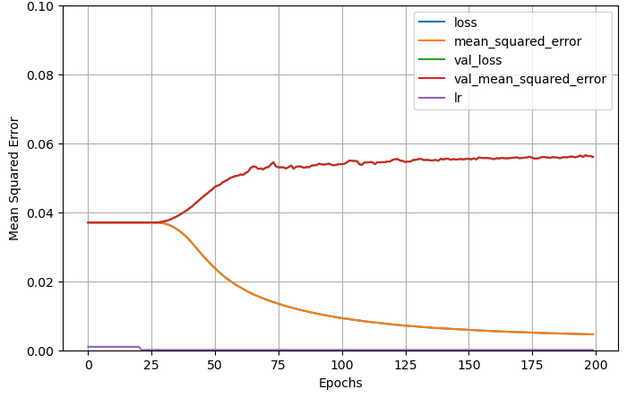
\includegraphics[ width=0.31\textwidth]{psf-PSFRecontructorSuperBigFC70000-1-evolution.png}}
			\hspace{\fill}
			\subfloat[Validation example]{%
			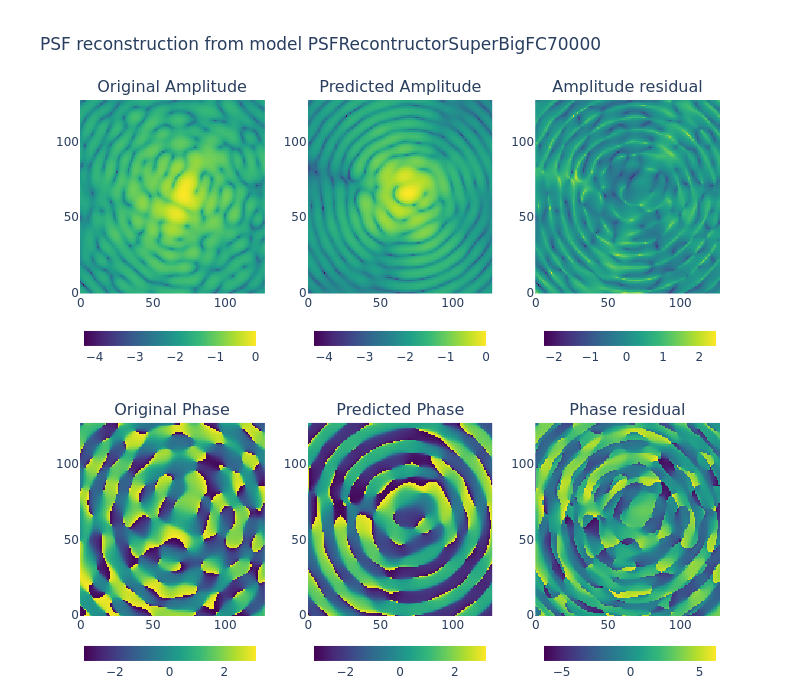
\includegraphics[ width=0.31\textwidth]{psf-PSFRecontructorSuperBigFC70000-1-val.png}}
			\hspace{\fill}
			\subfloat[Train example]{%
			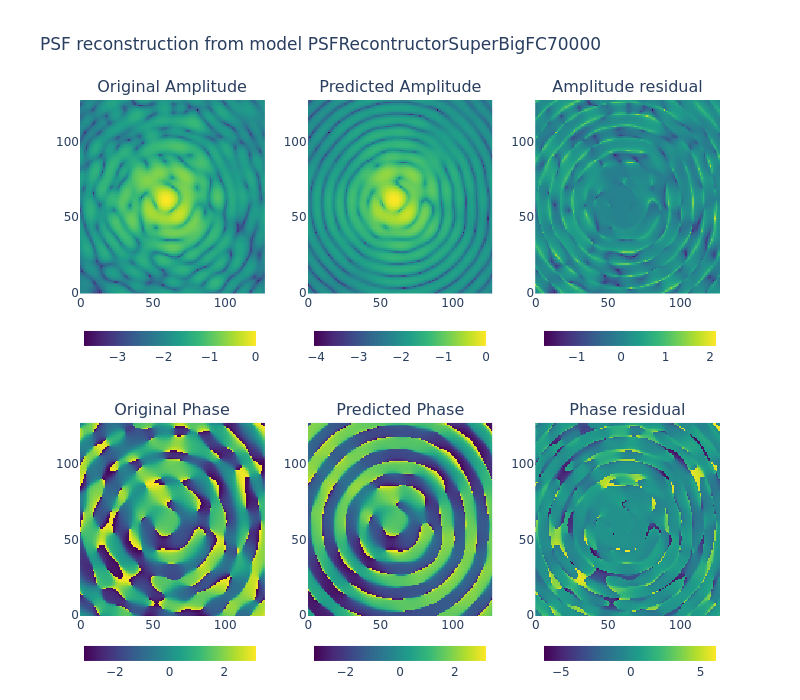
\includegraphics[ width=0.31\textwidth]{psf-PSFRecontructorSuperBigFC70000-1-train.png}}\\
			\caption{Results of training the model PSFRecontructorSuperBigFC70000-1}
		\end{figure*}
		
		\subparagraph{Cropped sized PSF}:\\
		\begin{lstlisting}	
        		-Train MSE: 0.008466990664601326
        		-Validation MSE: 0.20970138907432556
		\end{lstlisting}
		
		\begin{figure*}[ht!]
			\subfloat[Training Evolution]{%
			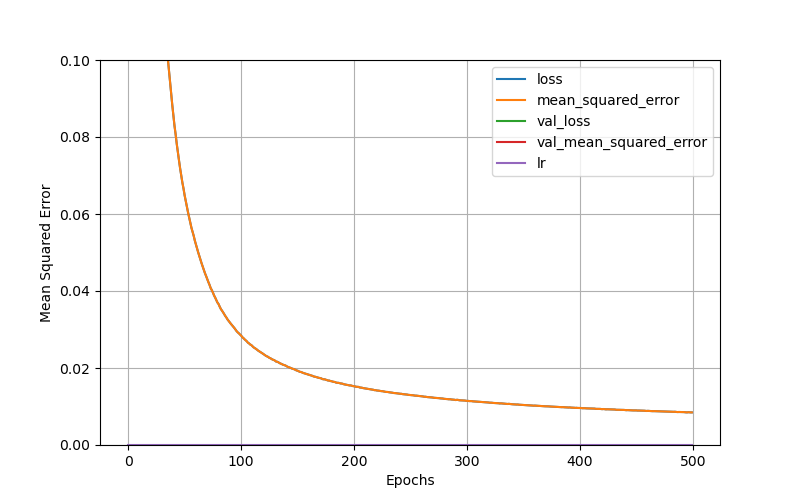
\includegraphics[ width=0.31\textwidth]{psf-CroppedBNFC70000-1-evolution.png}}
			\hspace{\fill}
			\subfloat[Validation example]{%
			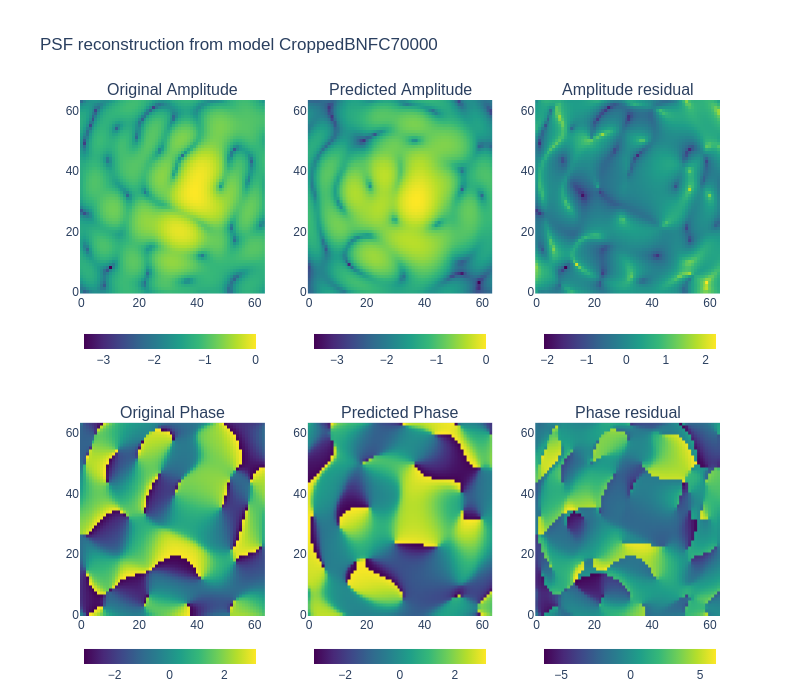
\includegraphics[ width=0.31\textwidth]{psf-CroppedBNFC70000-1-validation.png}}
			\hspace{\fill}
			\subfloat[Train example]{%
			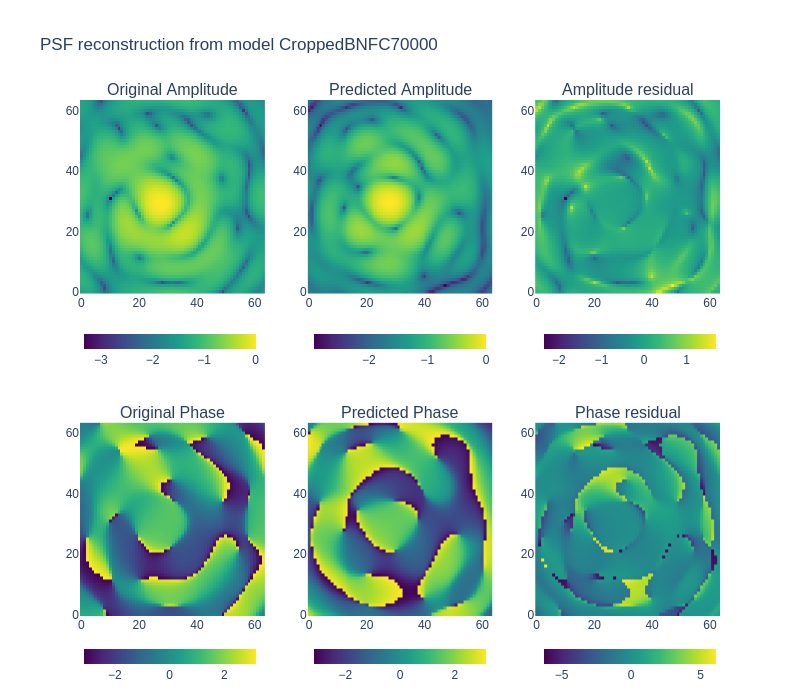
\includegraphics[ width=0.31\textwidth]{psf-CroppedBNFC70000-1-train.png}}\\
			\caption{Results of training the model PSFRecontructorSuperBigFC70000-1}
		\end{figure*}
	
\FloatBarrier

	\subsubsection{Zernike modes related models}
	
		\begin{figure*}[ht!]
				\centering	
				\subfloat[2 zernike mode PSF electric field model training]{%
					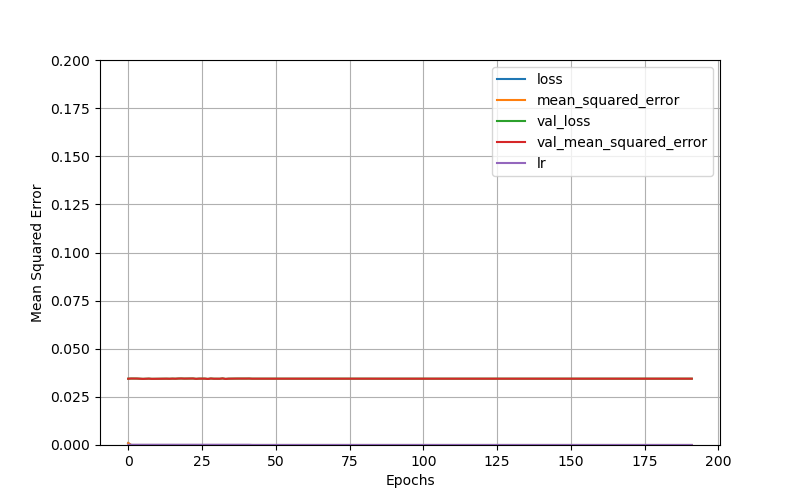
\includegraphics[width=0.22\textwidth]{psf-SuperBigZernike2MFC70000-1-evolution.png}}
				\hspace{\fill}
				\subfloat[2 zernike mode PSF intensity model training]{%
					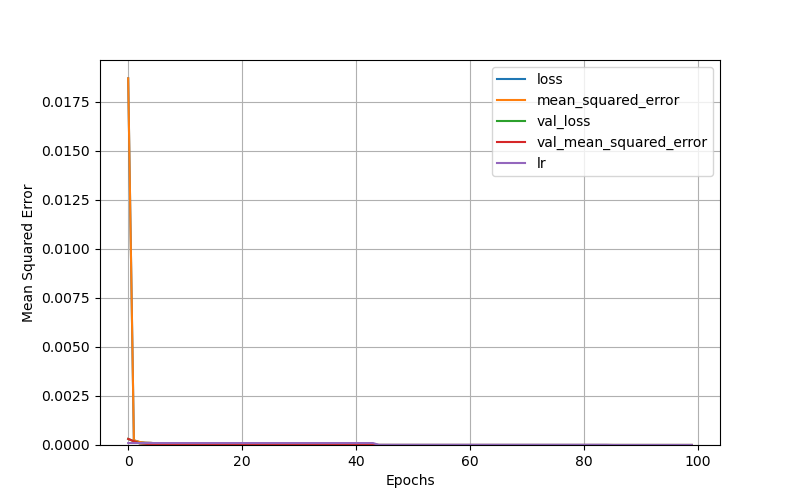
\includegraphics[width=0.22\textwidth]{psf-SuperBigZernike2MFCIntensity70000-1-evolution.png}}
				\hspace{\fill}	
				\subfloat[2 zernike mode cropped PSF electric field model training]{%
					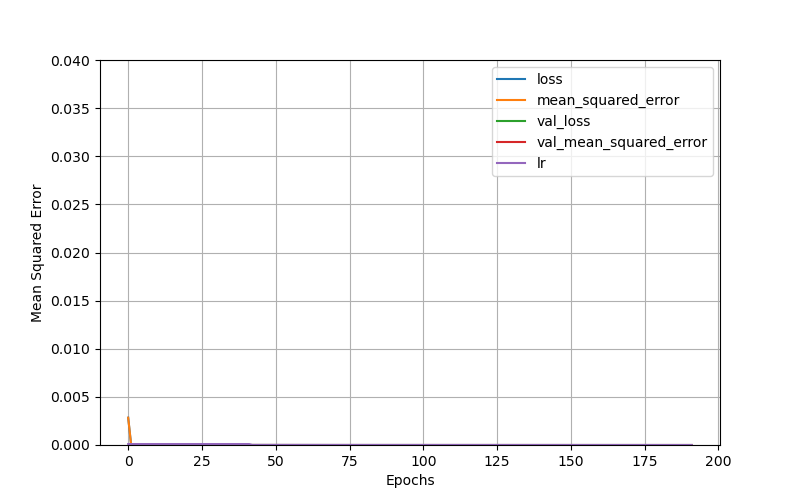
\includegraphics[width=0.22\textwidth]{psf-SuperBigCroppedZernike2MFC70000-1-evolution.png}}
				\hspace{\fill}	
				\subfloat[2 zernike mode cropped PSF intensity model training]{%
					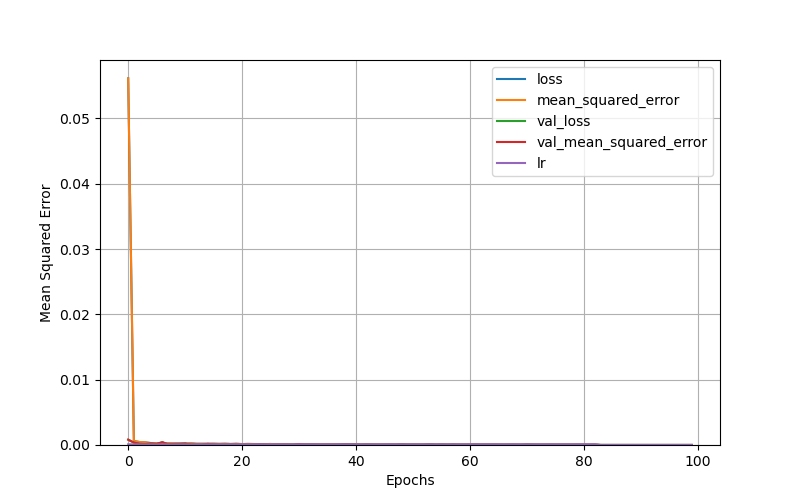
\includegraphics[width=0.22\textwidth]{psf-SuperBigCroppedZernike2MFCIntensity70000-1-evolution.png}}\\
					
				\subfloat[5 zernike mode PSF electric field model training]{%
					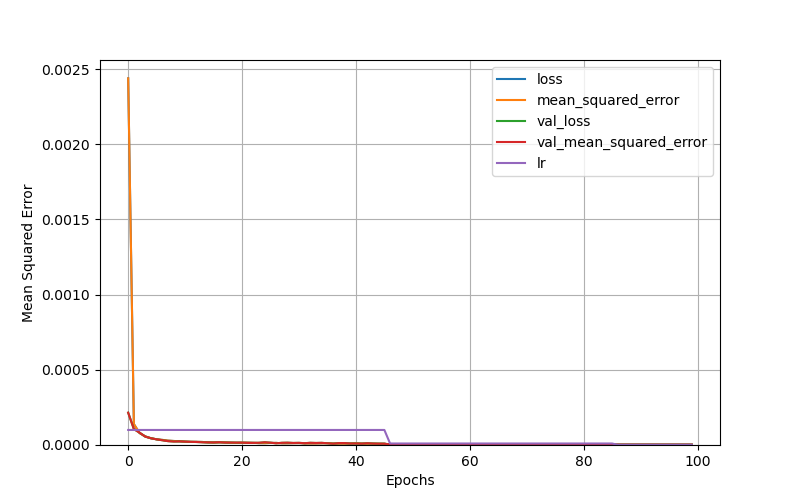
\includegraphics[width=0.22\textwidth]{psf-SuperBigZernike5MFC70000-1-evolution.png}}
				\hspace{\fill}
				\subfloat[5 zernike mode PSF intensity model training]{%
					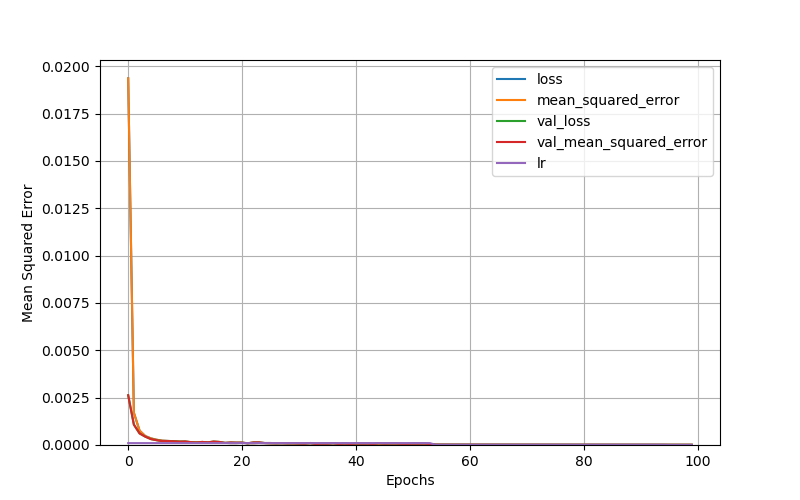
\includegraphics[width=0.22\textwidth]{psf-SuperBigZernike5MFCIntensity70000-1-evolution.png}}
				\hspace{\fill}	
				\subfloat[5 zernike mode cropped PSF electric field model training]{%
					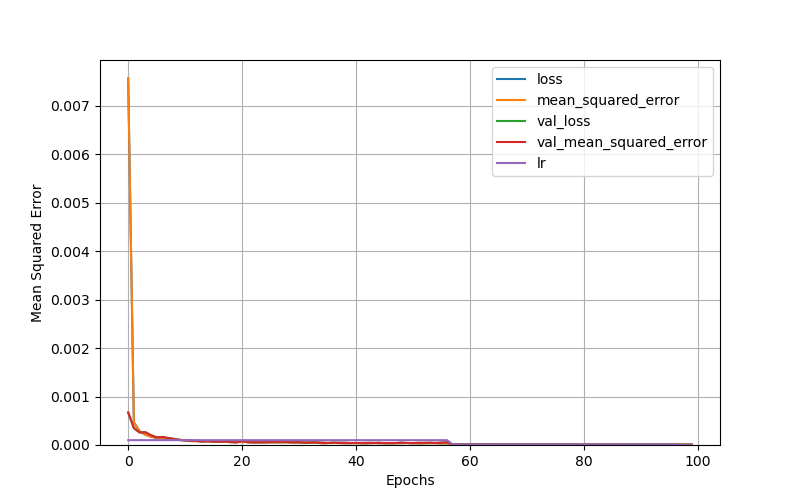
\includegraphics[width=0.22\textwidth]{psf-SuperBigCroppedZernike5MFC70000-1-evolution.png}}
				\hspace{\fill}	
				\subfloat[5 zernike mode cropped PSF intensity model training]{%
					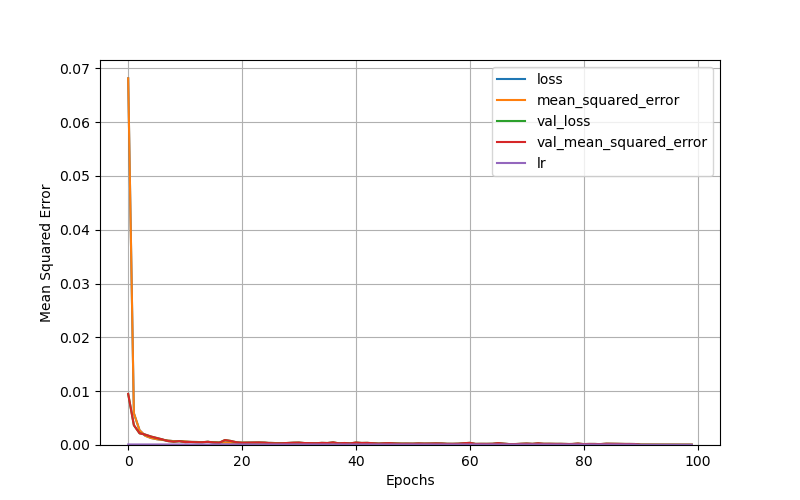
\includegraphics[width=0.22\textwidth]{psf-SuperBigCroppedZernike5MFCIntensity70000-1-evolution.png}}\\
					
				\subfloat[9 zernike mode PSF electric field model training]{%
					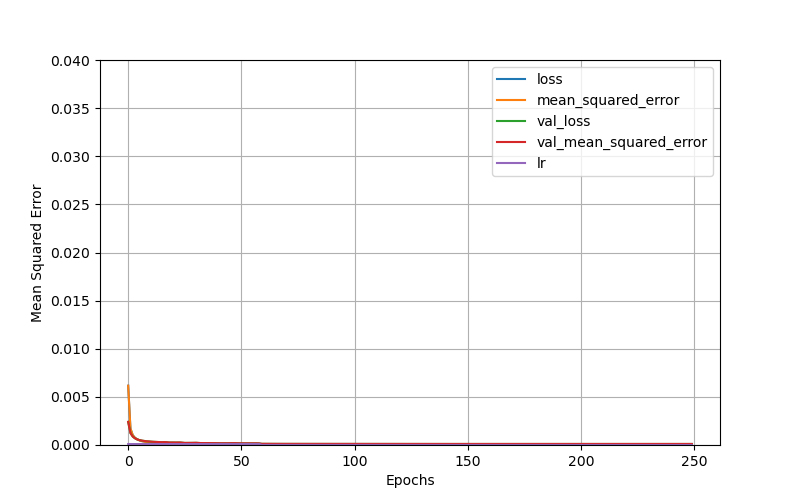
\includegraphics[width=0.22\textwidth]{psf-SuperBigZernike9MFC70000-1-evolution.png}}
				\hspace{\fill}
				\subfloat[9 zernike mode PSF intensity model training]{%
					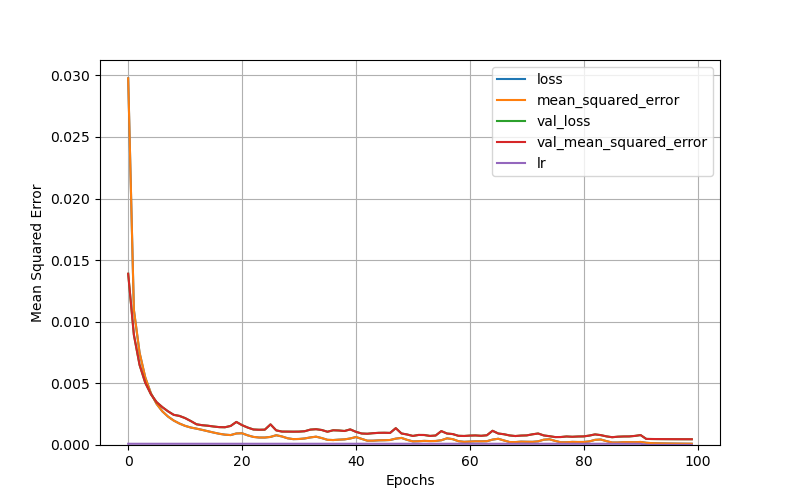
\includegraphics[width=0.22\textwidth]{psf-SuperBigZernike9MFCIntensity70000-1-evolution.png}}
				\hspace{\fill}	
				\subfloat[9 zernike mode cropped PSF electric field model training]{%
					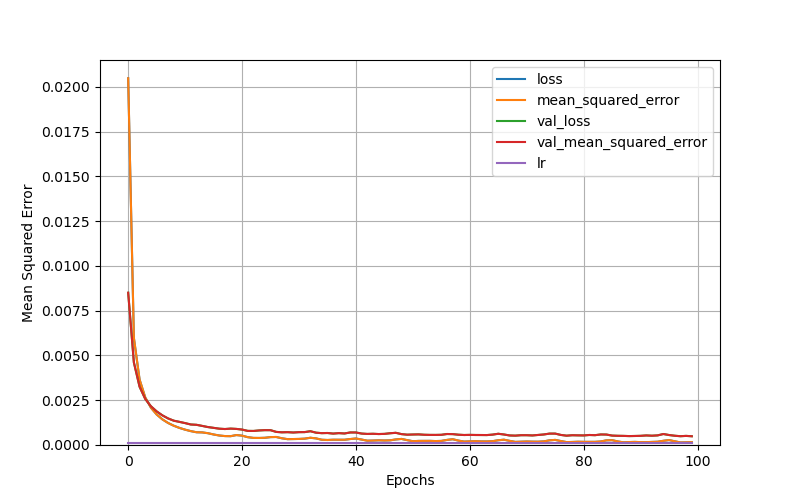
\includegraphics[width=0.22\textwidth]{psf-SuperBigCroppedZernike9MFC70000-1-evolution.png}}
				\hspace{\fill}	
				\subfloat[9 zernike mode cropped PSF intensity model training]{%
					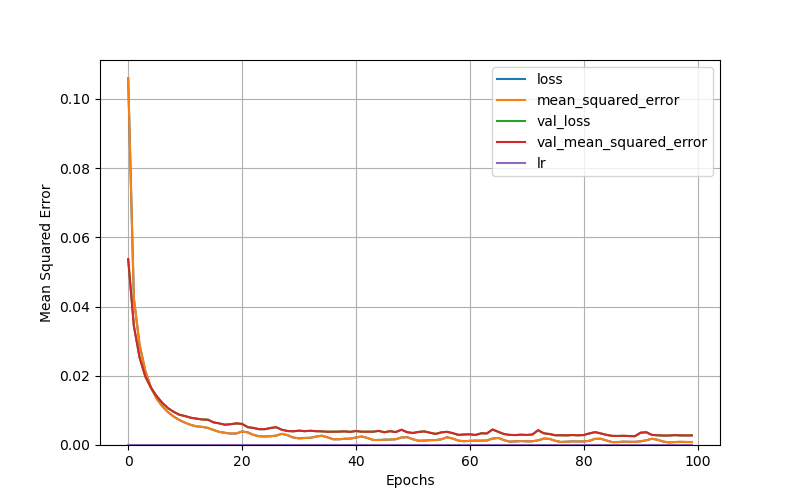
\includegraphics[width=0.22\textwidth]{psf-SuperBigCroppedZernike9MFCIntensity70000-1-evolution.png}}\\
					
				\subfloat[14 zernike mode PSF electric field model training]{%
					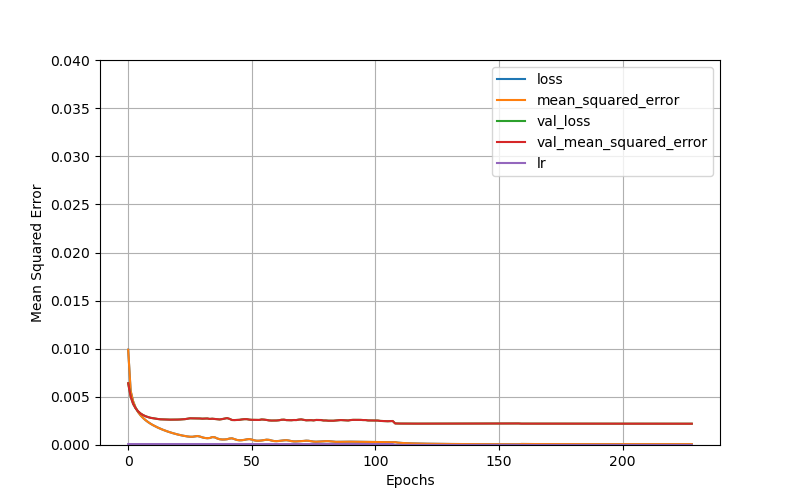
\includegraphics[width=0.22\textwidth]{psf-SuperBigZernike14MFC70000-1-evolution.png}}
				\hspace{\fill}
				\subfloat[14 zernike mode PSF intensity model training]{%
					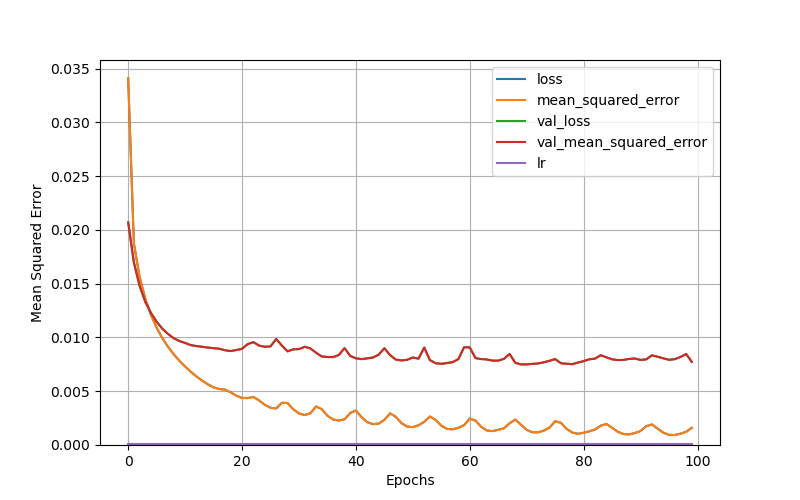
\includegraphics[width=0.22\textwidth]{psf-SuperBigZernike14MFCIntensity70000-1-evolution.png}}
				\hspace{\fill}	
				\subfloat[14 zernike mode cropped PSF electric field model training]{%
					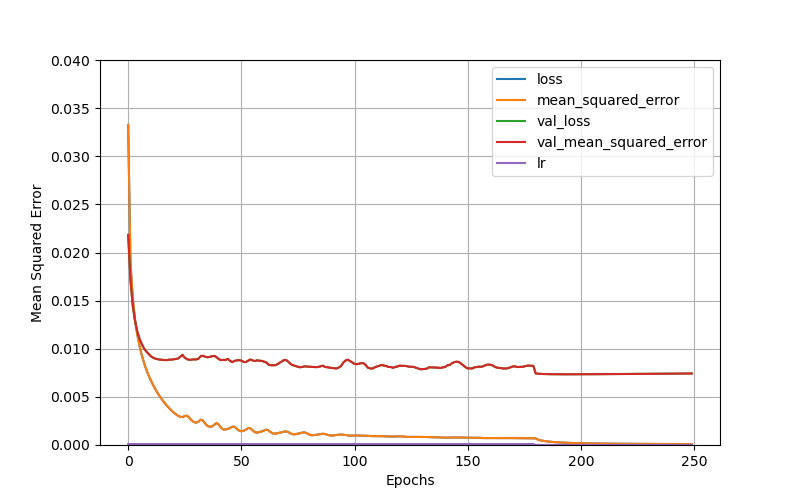
\includegraphics[width=0.22\textwidth]{psf-SuperBigCroppedZernike14MFC70000-1-evolution.png}}
				\hspace{\fill}	
				\subfloat[14 zernike mode cropped PSF intensity model training]{%
					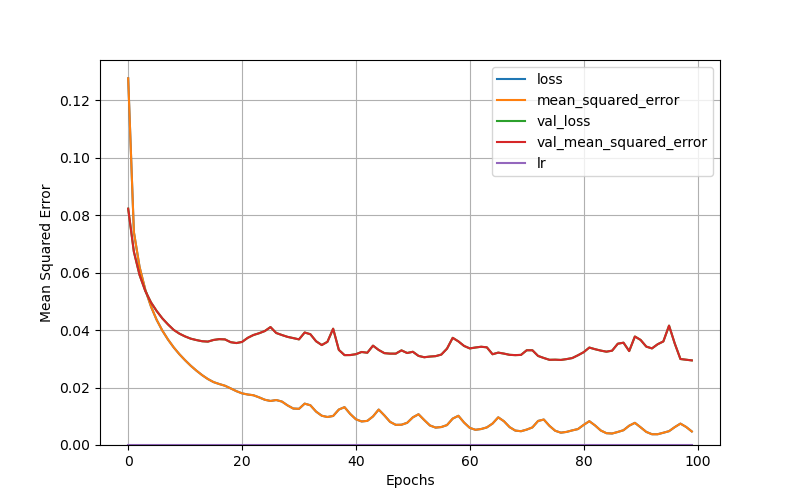
\includegraphics[width=0.22\textwidth]{psf-SuperBigCroppedZernike14MFCIntensity70000-1-evolution.png}}\\
					
				\subfloat[20 zernike mode PSF electric field model training]{%
					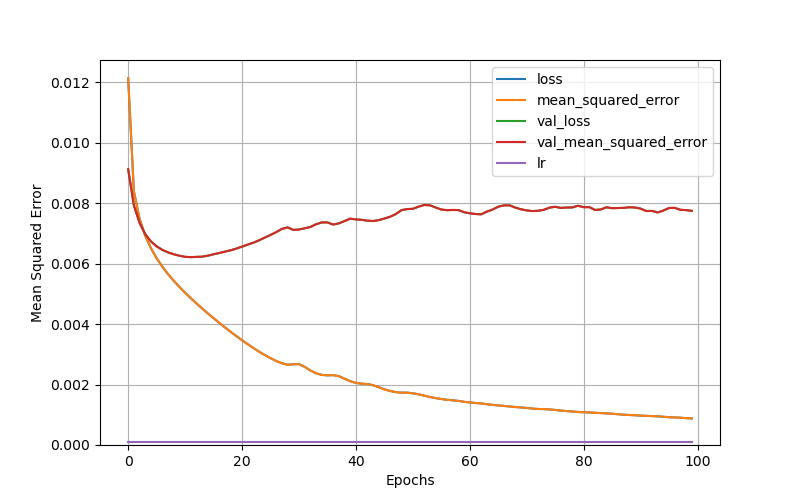
\includegraphics[width=0.22\textwidth]{psf-SuperBigZernike20MFC70000-1-evolution.png}}
				\hspace{\fill}
				\subfloat[20 zernike mode PSF intensity model training]{%
					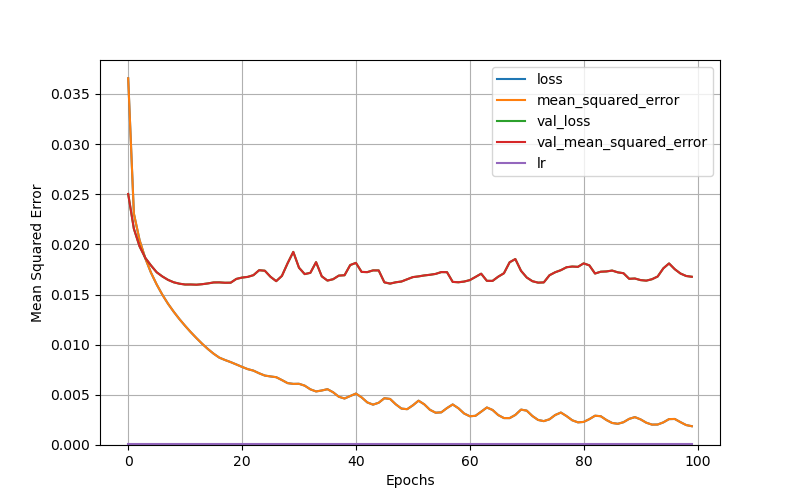
\includegraphics[width=0.22\textwidth]{psf-SuperBigZernike20MFCIntensity70000-1-evolution.png}}
				\hspace{\fill}	
				\subfloat[20 zernike mode cropped PSF electric field model training]{%
					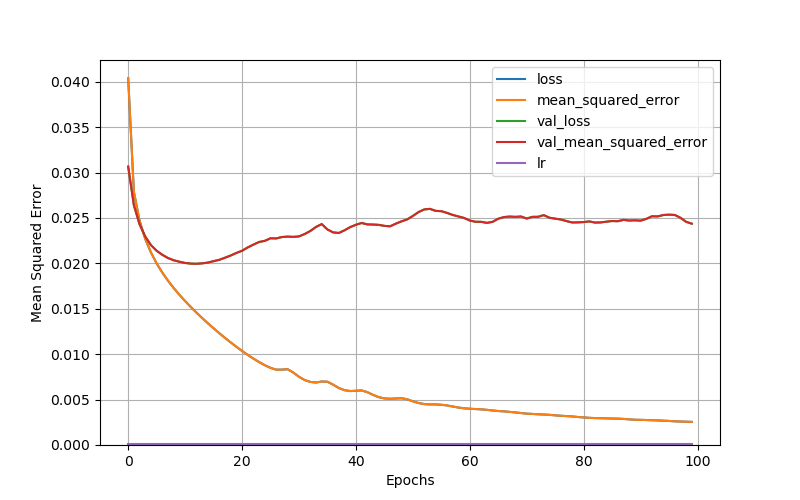
\includegraphics[width=0.22\textwidth]{psf-SuperBigCroppedZernike20MFC70000-1-evolution.png}}
				\hspace{\fill}	
				\subfloat[20 zernike mode cropped PSF intensity model training]{%
					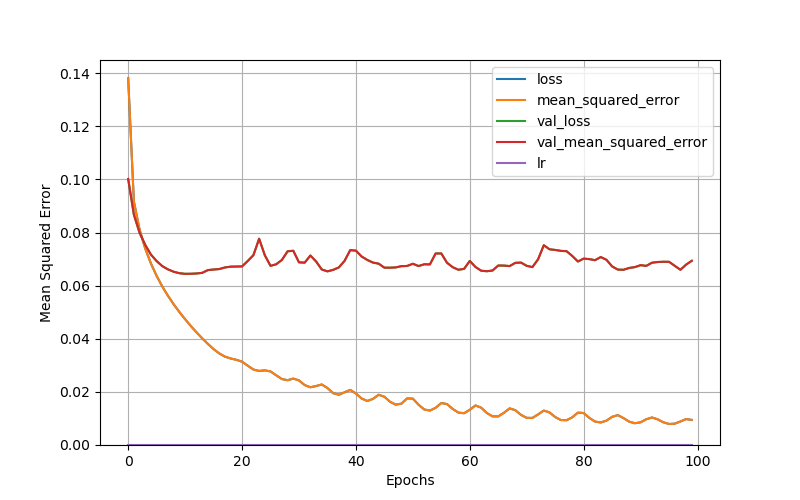
\includegraphics[width=0.22\textwidth]{psf-SuperBigCroppedZernike20MFCIntensity70000-1-evolution.png}}\\
			
			\caption{Training evolution comparison for the different Zernike datasets}
		\end{figure*}
		\FloatBarrier
		
		\subparagraph{2 modes PSF models MSE}:\\
		\begin{table}[h!]
			\centering
			\begin{tabular}{|c|c|c|c|c|}
				\hline
				  & \textbf{Electric field} & \textbf{Cropped electric field} & \textbf{Intensity} & \textbf{Cropped intensity}\\
				\hline
				\textbf{Train MSE} & 6.823e-8 & 1.770e-7 & 6.212e-7 & 2.646e-6 \\
				\hline
				\textbf{Val MSE} & 6.053e-8 & 1.450e-7 & 5.212e-7 & 1.880e-6 \\
				\hline
			\end{tabular}
		\caption{2 Zernike modes related models MSE}
		\end{table}
		\FloatBarrier
		
		\subparagraph{5 modes PSF models MSE}:\\
		\begin{table}[h!]
			\centering
			\begin{tabular}{|c|c|c|c|c|}
				\hline
				  & \textbf{Electric field} & \textbf{Cropped electric field} & \textbf{Intensity} & \textbf{Cropped intensity}\\
				\hline
				\textbf{Train MSE} & 1.753e-6 & 4.443e-6 & 6.019e-6 & 3.044e-5\\
				\hline
				\textbf{Val MSE} & 2.529e-6 & 7.328e-6 & 1.142e-6 & 4.700e-5\\
				\hline
			\end{tabular}
		\caption{5 Zernike modes related models MSE}
		\end{table}
		\FloatBarrier
		
		\subparagraph{9 modes PSF models MSE}:\\
		\begin{table}[h!]
			\centering
			\begin{tabular}{|c|c|c|c|c|}
				\hline
				  & \textbf{Electric field} & \textbf{Cropped electric field} & \textbf{Intensity} & \textbf{Cropped intensity}\\
				\hline
				\textbf{Train MSE} & 1.825e-5 & 1.599e-4 & 1.025e-4 & 8.590e-4\\
				\hline
				\textbf{Val MSE} & 1.025e-4 & 4.883e-4 & 4.667e-4 & 2.770e-3\\
				\hline
			\end{tabular}
		\caption{9 Zernike modes related models MSE}
		\end{table}
		\FloatBarrier
		
		\subparagraph{14 modes PSF models MSE}:\\
		\begin{table}[h!]
			\centering
			\begin{tabular}{|c|c|c|c|c|}
				\hline
				  & \textbf{Electric field} & \textbf{Cropped electric field} & \textbf{Intensity} & \textbf{Cropped intensity}\\
				\hline
				\textbf{Train MSE} & 3.085e-4 & 9.827e-4 & 1.597e-3 & 4.715e-3\\
				\hline
				\textbf{Val MSE} & 2.602e-3 & 8.197e-3 & 7.773e-3 & 0.0294\\
				\hline
			\end{tabular}
		\caption{14 Zernike modes related models MSE}
		\end{table}
		\FloatBarrier
		
		\subparagraph{20 modes PSF models MSE}:\\
		\begin{table}[h!]
			\centering
			\begin{tabular}{|c|c|c|c|c|}
				\hline
				  & \textbf{Electric field} & \textbf{Cropped electric field} & \textbf{Intensity} & \textbf{Cropped intensity}\\
				\hline
				\textbf{Train MSE} & 8.804e-4 & 2.546e-3 & 1.872e-3 & 9.445e-3 \\
				\hline
				\textbf{Val MSE} & 7.74e-3 & 0.024 & 0.0167 & 0.069 \\
				\hline
			\end{tabular}
		\caption{20 Zernike modes related models MSE}
		\end{table}
		\FloatBarrier
		
		A summary of the MSE evolution over the Zernike PSFs datasets is shown below. The fact that the validation MSE for 2 modes is the worse may be because the neural network is not able to understand traslations.
		\begin{figure*}[ht!]
			\centering
			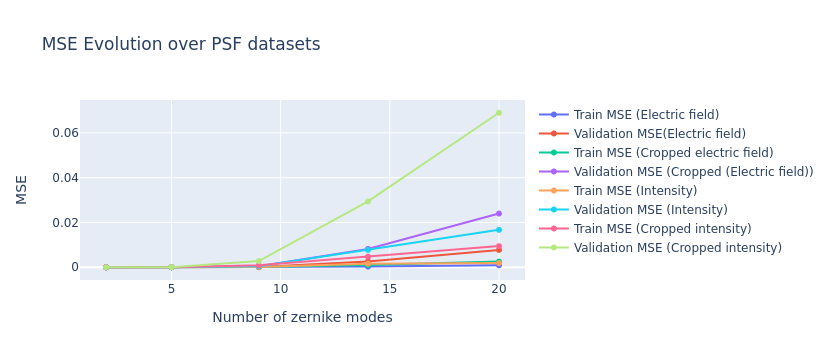
\includegraphics[width=\textwidth]{pid-mseevolutionzernikedatasets}
			\caption{MSE evolution over the Zernike PSFs datasets}
		\end{figure*}
		
		\begin{figure*}[ht!]
			\centering
			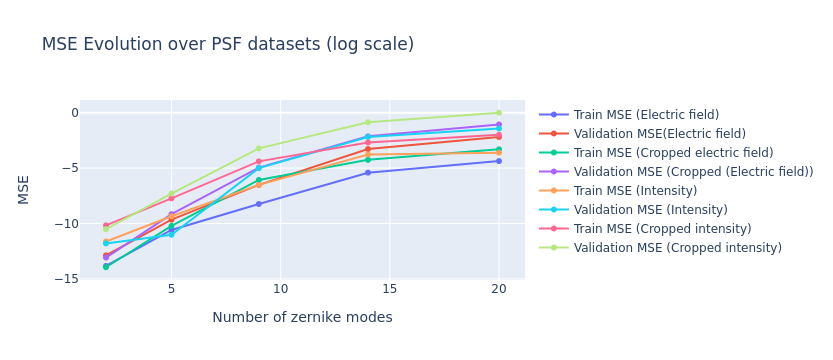
\includegraphics[width=\textwidth]{pid-mseevolutionzernikedatasetslog}
			\caption{MSE evolution over the Zernike PSFs datasets in logarithmic scale}
		\end{figure*}
		
		\FloatBarrier
		
		\subparagraph{Model output examples}:\\
		\begin{figure*}[ht!]
			\subfloat[Train example from electric field model]{%
				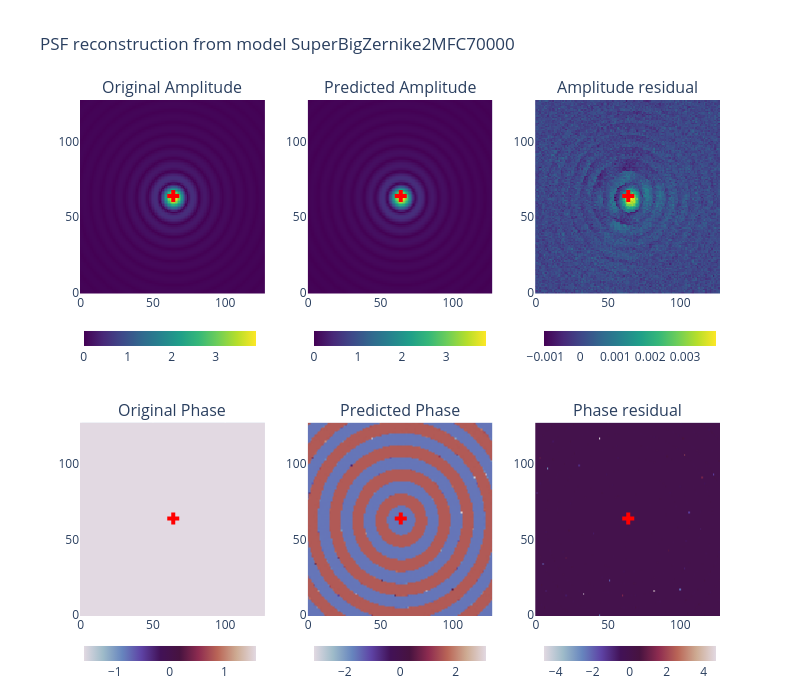
\includegraphics[width=0.45\textwidth]{psf-SuperBigZernike2MFC70000-1-train.png}}
			\hspace{\fill}
			\subfloat[Validation example from electric field model]{%
				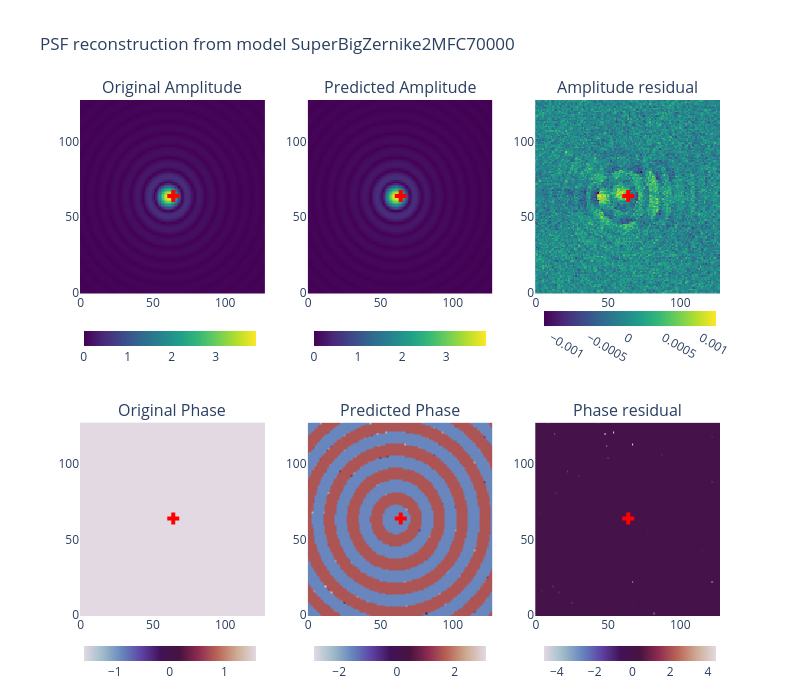
\includegraphics[ width=0.45\textwidth]{psf-SuperBigZernike2MFC70000-1-validation.png}}\\
			
			\subfloat[Train example from intensity model]{%
				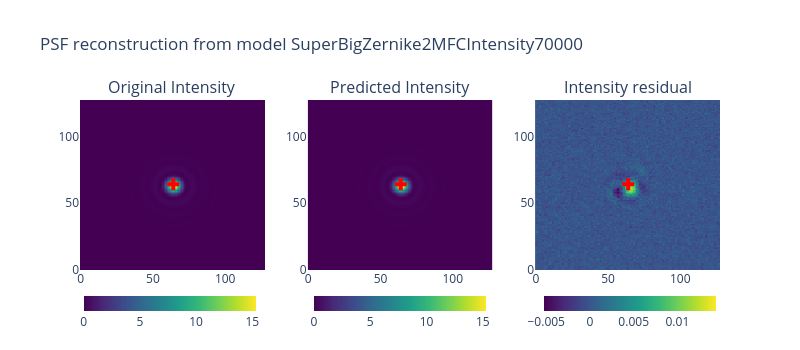
\includegraphics[ width=0.45\textwidth]{psf-SuperBigZernike2MFCIntensity70000-1-train.png}}
			\hspace{\fill}
			\subfloat[Validation example from intensity model]{%
				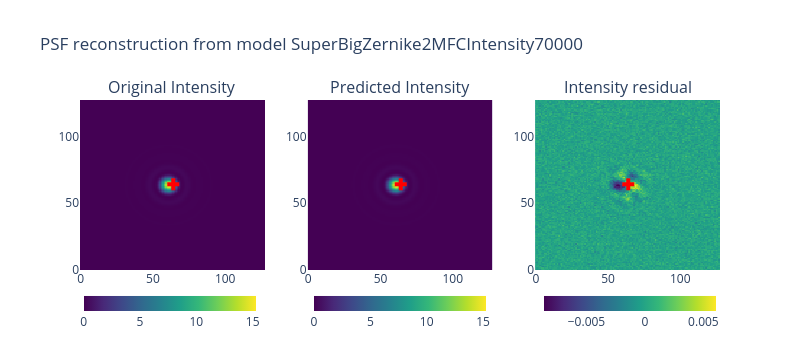
\includegraphics[ width=0.45\textwidth]{psf-SuperBigZernike2MFCIntensity70000-1-validation.png}}\\
				
			\subfloat[Train example from cropped electric field model]{%
				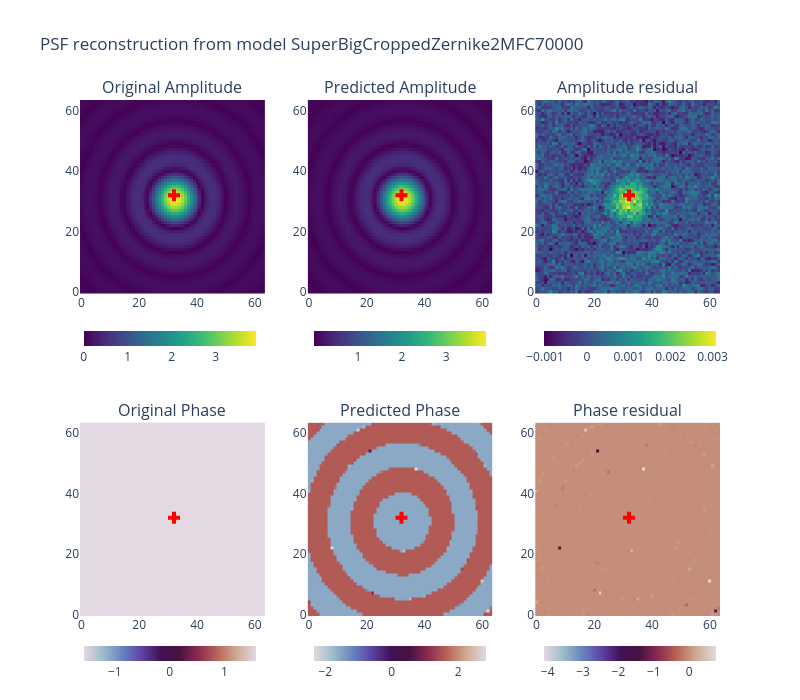
\includegraphics[width=0.45\textwidth]{psf-SuperBigCroppedZernike2MFC70000-1-train.png}}
			\hspace{\fill}
			\subfloat[Validation example cropped from electric field model]{%
				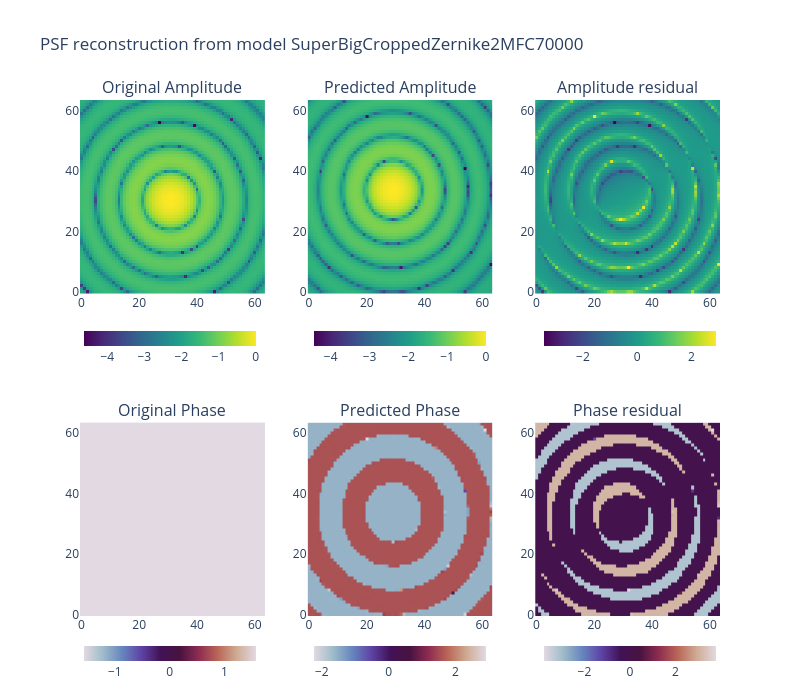
\includegraphics[ width=0.45\textwidth]{psf-SuperBigCroppedZernike2MFC70000-1-validation.png}}\\
			
			\subfloat[Train example from cropped intensity model]{%
				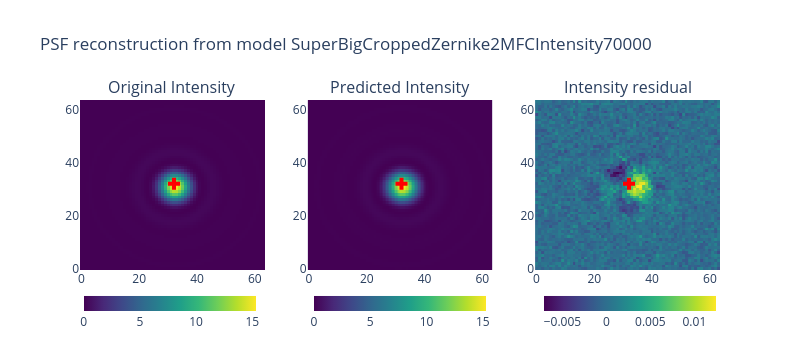
\includegraphics[ width=0.45\textwidth]{psf-SuperBigCroppedZernike2MFCIntensity70000-1-train.png}}
			\hspace{\fill}
			\subfloat[Validation example from cropped model]{%
				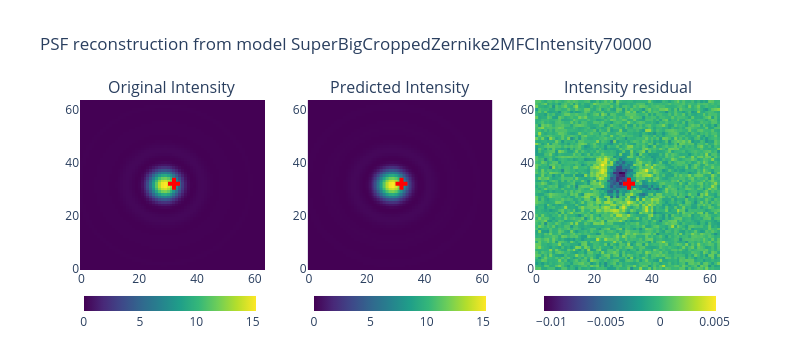
\includegraphics[ width=0.45\textwidth]{psf-SuperBigCroppedZernike2MFCIntensity70000-1-validation.png}}\\
				
			\caption{Model outputs for 2 mode PSF datasets}
		\end{figure*}
		\FloatBarrier
		
		
		\begin{figure*}[ht!]
			\subfloat[Train example from electric field model]{%
				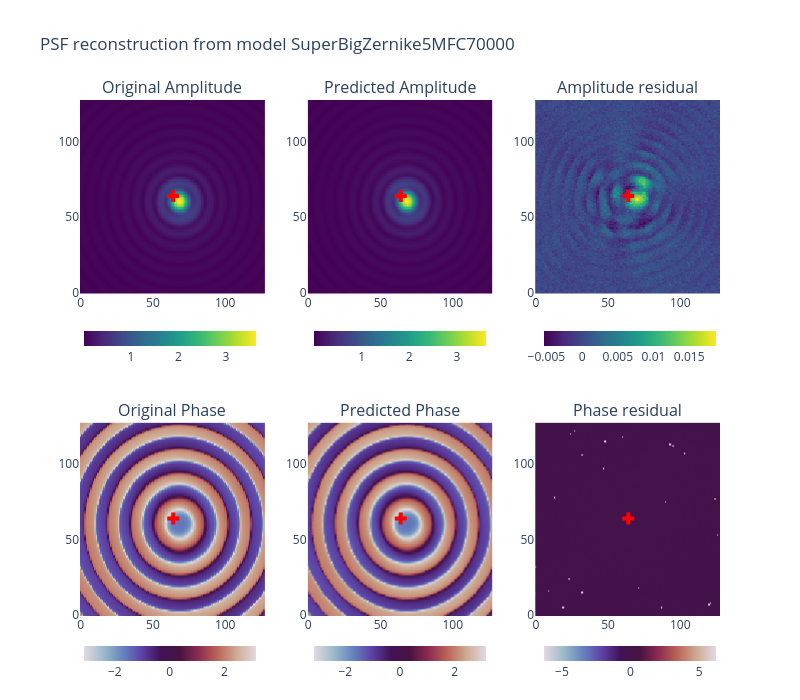
\includegraphics[width=0.45\textwidth]{psf-SuperBigZernike5MFC70000-1-train.png}}
			\hspace{\fill}
			\subfloat[Validation example from electric field model]{%
				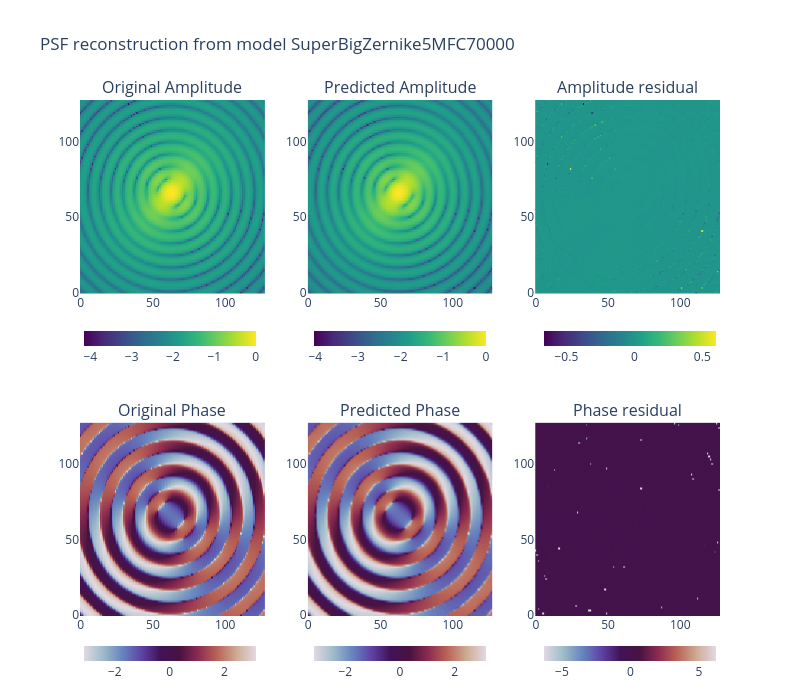
\includegraphics[ width=0.45\textwidth]{psf-SuperBigZernike5MFC70000-1-validation.png}}\\
			
			\subfloat[Train example from intensity model]{%
				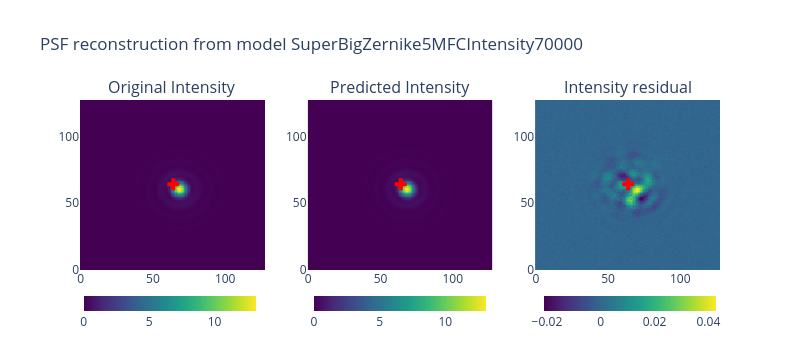
\includegraphics[ width=0.45\textwidth]{psf-SuperBigZernike5MFCIntensity70000-1-train.png}}
			\hspace{\fill}
			\subfloat[Validation example from intensity model]{%
				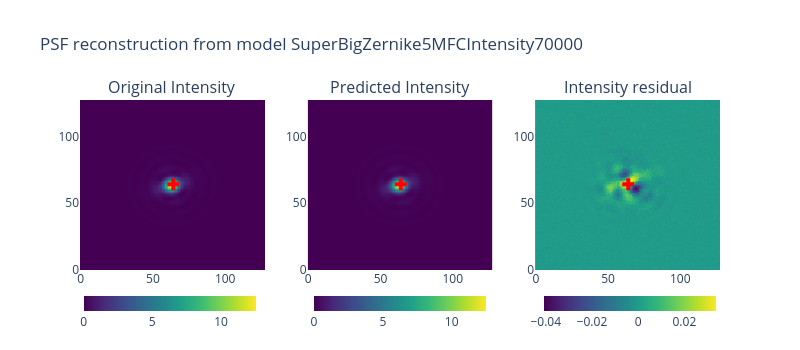
\includegraphics[ width=0.45\textwidth]{psf-SuperBigZernike5MFCIntensity70000-1-validation.png}}\\
				
			\subfloat[Train example from cropped electric field model]{%
				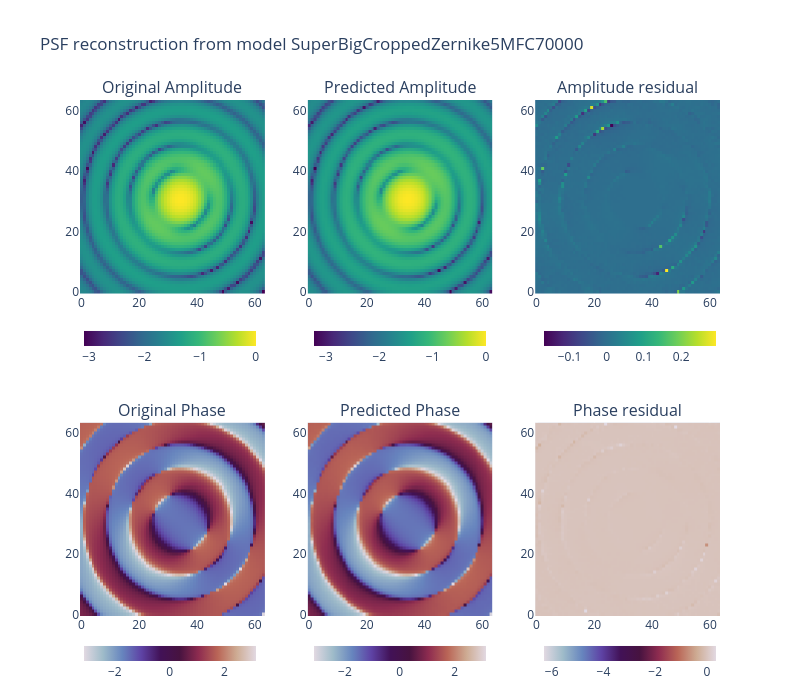
\includegraphics[width=0.45\textwidth]{psf-SuperBigCroppedZernike5MFC70000-1-train.png}}
			\hspace{\fill}
			\subfloat[Validation example cropped from electric field model]{%
				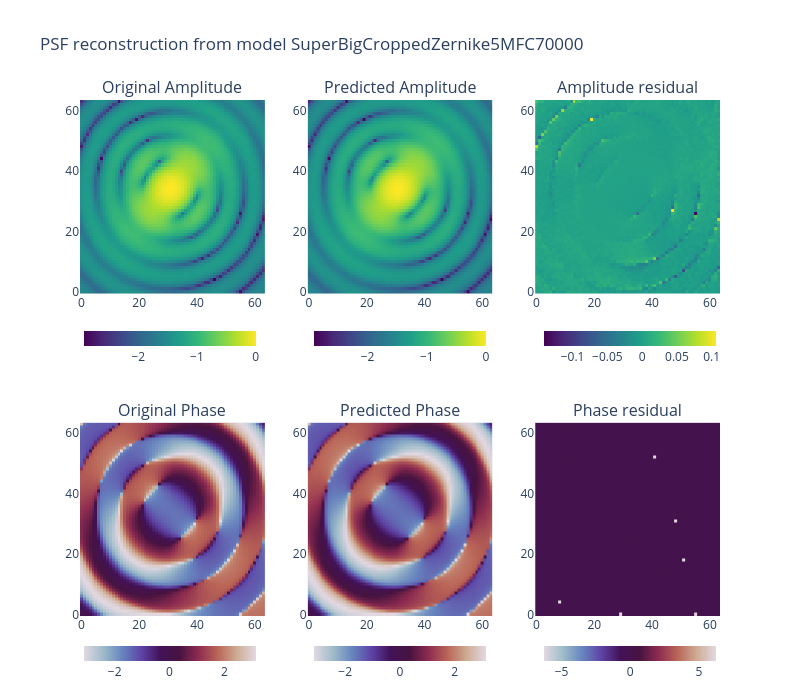
\includegraphics[ width=0.45\textwidth]{psf-SuperBigCroppedZernike5MFC70000-1-validation.png}}\\
			
			\subfloat[Train example from cropped intensity model]{%
				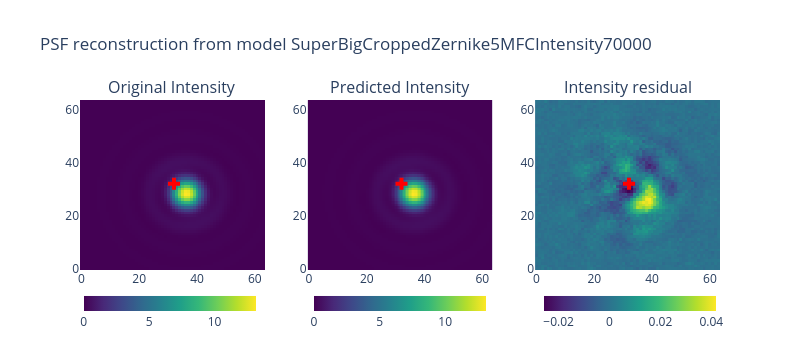
\includegraphics[ width=0.45\textwidth]{psf-SuperBigCroppedZernike5MFCIntensity70000-1-train.png}}
			\hspace{\fill}
			\subfloat[Validation example from cropped model]{%
				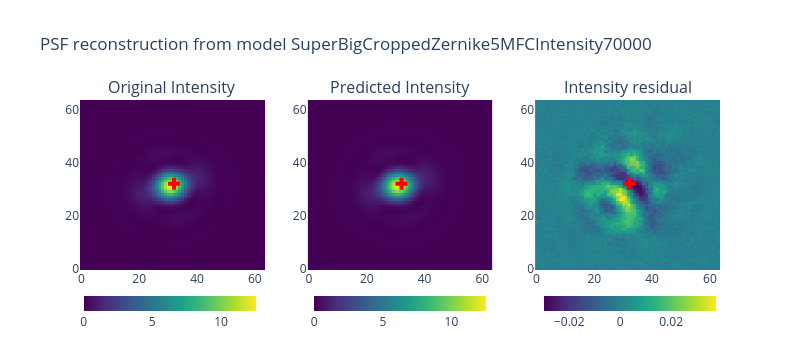
\includegraphics[ width=0.45\textwidth]{psf-SuperBigCroppedZernike5MFCIntensity70000-1-validation.png}}\\
				
			\caption{Model outputs for 5 mode PSF datasets}
		\end{figure*}
		\FloatBarrier
		
		
		\begin{figure*}[ht!]
			\subfloat[Train example from electric field model]{%
				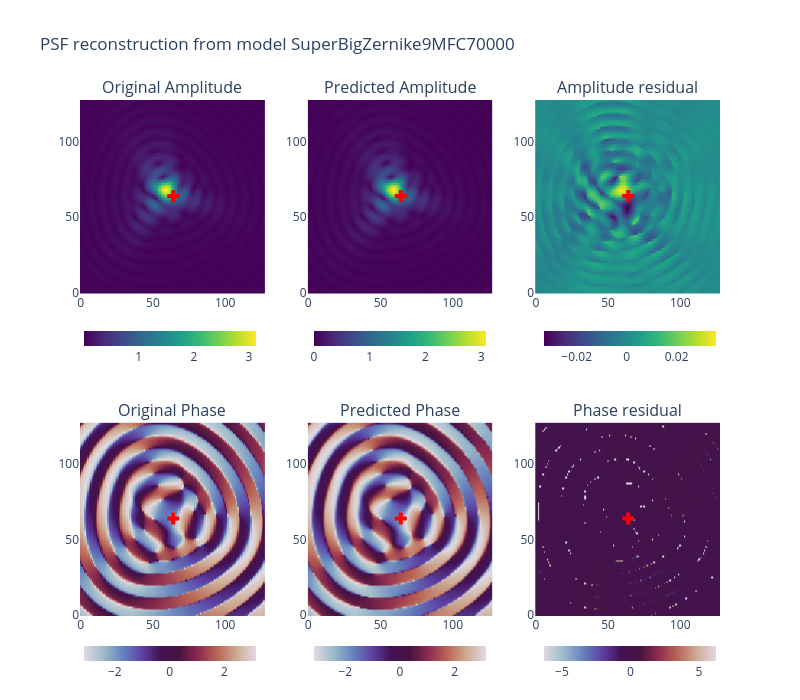
\includegraphics[width=0.45\textwidth]{psf-SuperBigZernike9MFC70000-1-train.png}}
			\hspace{\fill}
			\subfloat[Validation example from electric field model]{%
				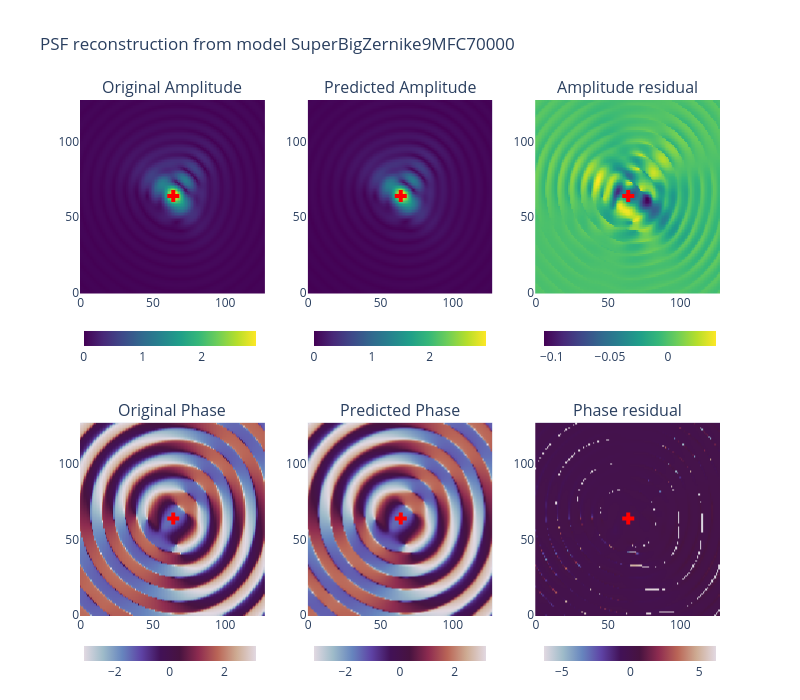
\includegraphics[ width=0.45\textwidth]{psf-SuperBigZernike9MFC70000-1-validation.png}}\\
			
			\subfloat[Train example from intensity model]{%
				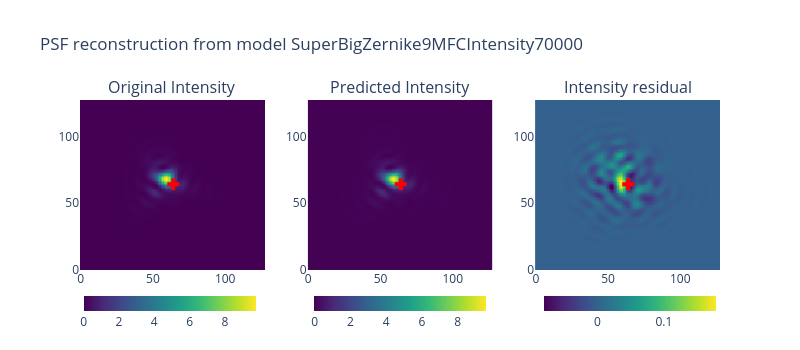
\includegraphics[ width=0.45\textwidth]{psf-SuperBigZernike9MFCIntensity70000-1-train.png}}
			\hspace{\fill}
			\subfloat[Validation example from intensity model]{%
				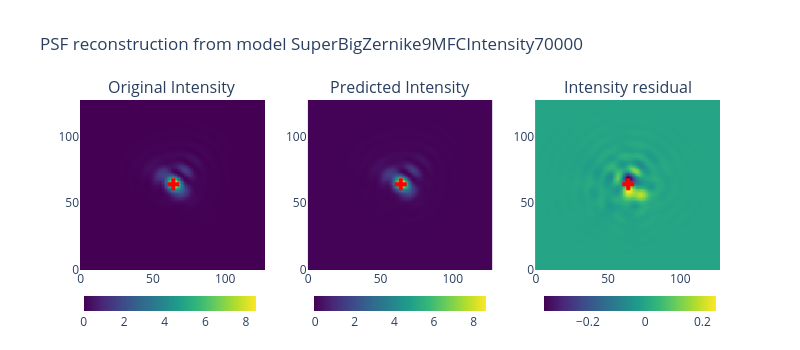
\includegraphics[ width=0.45\textwidth]{psf-SuperBigZernike9MFCIntensity70000-1-validation.png}}\\
				
			\subfloat[Train example from cropped electric field model]{%
				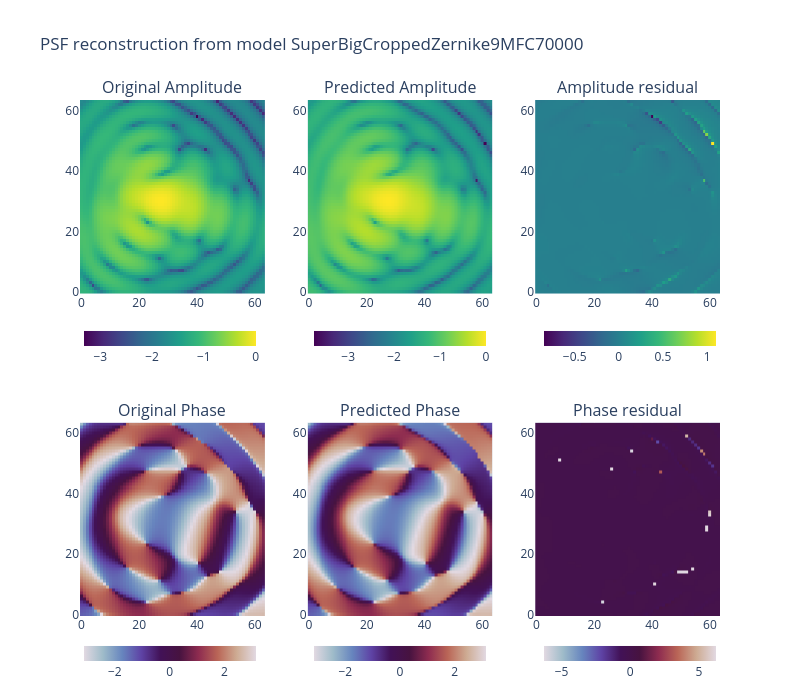
\includegraphics[width=0.45\textwidth]{psf-SuperBigCroppedZernike9MFC70000-1-train.png}}
			\hspace{\fill}
			\subfloat[Validation example cropped from electric field model]{%
				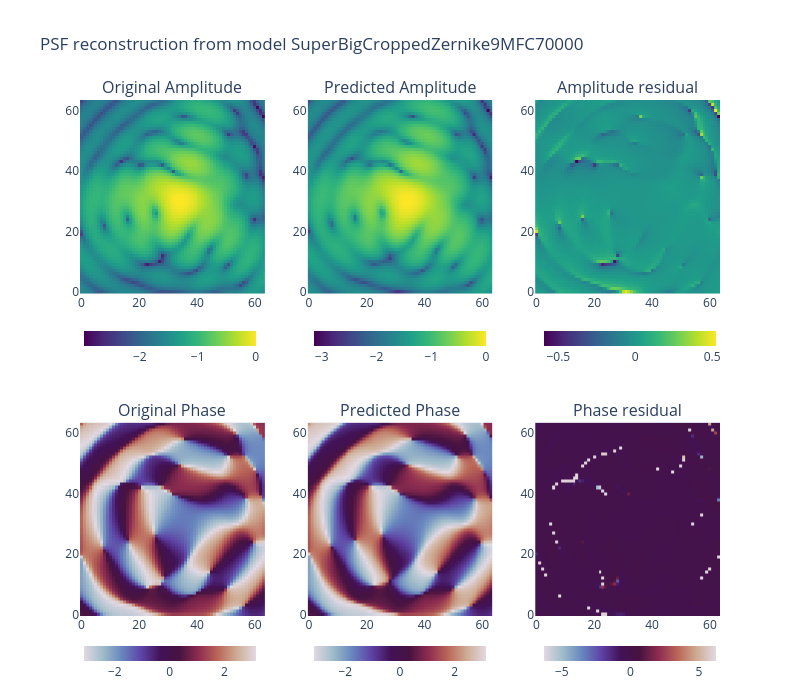
\includegraphics[ width=0.45\textwidth]{psf-SuperBigCroppedZernike9MFC70000-1-validation.png}}\\
			
			\subfloat[Train example from cropped intensity model]{%
				\includegraphics[ width=0.45\textwidth]{psf-SuperBigCroppedZernike9MFCIntensity70000-1-train.png}}
			\hspace{\fill}
			\subfloat[Validation example from cropped model]{%
				\includegraphics[ width=0.45\textwidth]{psf-SuperBigCroppedZernike9MFCIntensity70000-1-validation.png}}\\
				
			\caption{Model outputs for 9 mode PSF datasets}
		\end{figure*}
		\FloatBarrier
		
		
		\begin{figure*}[ht!]
			\subfloat[Train example from electric field model]{%
				\includegraphics[width=0.45\textwidth]{psf-SuperBigZernike14MFC70000-1-train.png}}
			\hspace{\fill}
			\subfloat[Validation example from electric field model]{%
				\includegraphics[ width=0.45\textwidth]{psf-SuperBigZernike14MFC70000-1-validation.png}}\\
			
			\subfloat[Train example from intensity model]{%
				\includegraphics[ width=0.45\textwidth]{psf-SuperBigZernike14MFCIntensity70000-1-train.png}}
			\hspace{\fill}
			\subfloat[Validation example from intensity model]{%
				\includegraphics[ width=0.45\textwidth]{psf-SuperBigZernike14MFCIntensity70000-1-validation.png}}\\
				
			\subfloat[Train example from cropped electric field model]{%
				\includegraphics[width=0.45\textwidth]{psf-SuperBigCroppedZernike14MFC70000-1-train.png}}
			\hspace{\fill}
			\subfloat[Validation example cropped from electric field model]{%
				\includegraphics[ width=0.45\textwidth]{psf-SuperBigCroppedZernike14MFC70000-1-validation.png}}\\
			
			\subfloat[Train example from cropped intensity model]{%
				\includegraphics[ width=0.45\textwidth]{psf-SuperBigCroppedZernike14MFCIntensity70000-1-train.png}}
			\hspace{\fill}
			\subfloat[Validation example from cropped model]{%
				\includegraphics[ width=0.45\textwidth]{psf-SuperBigCroppedZernike14MFCIntensity70000-1-validation.png}}\\
				
			\caption{Model outputs for 14 mode PSF datasets}
		\end{figure*}
		\FloatBarrier
		
		
		\begin{figure*}[ht!]
			\subfloat[Train example from electric field model]{%
				\includegraphics[width=0.45\textwidth]{psf-SuperBigZernike20MFC70000-1-train.png}}
			\hspace{\fill}
			\subfloat[Validation example from electric field model]{%
				\includegraphics[ width=0.45\textwidth]{psf-SuperBigZernike20MFC70000-1-validation.png}}\\
			
			\subfloat[Train example from intensity model]{%
				\includegraphics[ width=0.45\textwidth]{psf-SuperBigZernike20MFCIntensity70000-1-train.png}}
			\hspace{\fill}
			\subfloat[Validation example from intensity model]{%
				\includegraphics[ width=0.45\textwidth]{psf-SuperBigZernike20MFCIntensity70000-1-validation.png}}\\
				
			\subfloat[Train example from cropped electric field model]{%
				\includegraphics[width=0.45\textwidth]{psf-SuperBigCroppedZernike20MFC70000-1-train.png}}
			\hspace{\fill}
			\subfloat[Validation example cropped from electric field model]{%
				\includegraphics[ width=0.45\textwidth]{psf-SuperBigCroppedZernike20MFC70000-1-validation.png}}\\
			
			\subfloat[Train example from cropped intensity model]{%
				\includegraphics[ width=0.45\textwidth]{psf-SuperBigCroppedZernike20MFCIntensity70000-1-train.png}}
			\hspace{\fill}
			\subfloat[Validation example from cropped model]{%
				\includegraphics[ width=0.45\textwidth]{psf-SuperBigCroppedZernike20MFCIntensity70000-1-validation.png}}\\
				
			\caption{Model outputs for 20 mode PSF datasets}
		\end{figure*}
		\FloatBarrier
		
		
		